% template.tex, dated April 5 2013
% This is a template file for Annual Reviews 1 column Journals
%
% Compilation using ar-1col.cls' - version 1.0, Aptara Inc.
% (c) 2013 AR
%
% Steps to compile: latex latex latex
%
% For tracking purposes => this is v1.0 - Apr. 2013
\newcommand{\g}[1]{{\color{blue}{#1}}}
\newcommand{\plr}[1]{{\color{magenta}{#1}}}
\newcommand{\E}{\mathbb{E}}
\documentclass{ar-1col}
\addtolength{\voffset}{-0.5in}

\usepackage{subcaption}
\usepackage{amsfonts}

\setcounter{secnumdepth}{4}

% Metadata Information
\jname{Xxxx. Xxx. Xxx. Xxx.}
\jvol{AA}
\jyear{YYYY}
\doi{10.1146/((please add article doi))}


% Document starts
\begin{document}

% Page header
\markboth{Bradburd and Ralph}{Spatial Population Genetics}

% Title
\title{Spatial Population Genetics: It's About Time}


%Authors, affiliations address.
\author{Gideon S. Bradburd,$^1$ Peter L. Ralph$^2$
\affil{$^1$Ecology, Evolutionary Biology, and Behavior Group, Department of Integrative Biology, Michigan State University, East Lansing, MI, USA, 48824;
email: bradburd@msu.edu}
\affil{$^2$Institute of Ecology and Evolution, Departments of Mathematics and Biology, University of Oregon, Eugene, OR 97403}
}

%Abstract
\begin{abstract}
Abstract text, approximately 150 words.
\end{abstract}

%Keywords, etc.
\begin{keywords}
population genetics, isolation by distance, population structure, local adaptation
%keywords, separated by comma, no full stop, lowercase
\end{keywords}
\maketitle

%Table of Contents
\tableofcontents


% Heading 1
\section{Introduction}

The field of population genetics is shaped by a continuing conversation
between theory, methods, and data.
We design experiments and collect empirical data 
with the methods we will use to analyze them in mind; 
in turn, those methods are based on theory 
that was developed to explain observations from empirical data.
With some notable exceptions,
especially the work of Sewall Wright (e.g., refs) 
and Gustave Mal\'ecot (e.g., refs)
\g{, and later Monty Slatkin (e.g., refs),}
much of the early body of theory was focused on 
developing expectations for discrete populations.
The focus theory maintained on results in discrete populations 
both informed and was informed by early empirical datasets, 
most of which 
(although again, 
with some notable exceptions (e.g., fly clines, dobzhansky 1947)),
were well-described as discrete populations --
e.g., samples of flies in a vial \cite{Lewontin1974}.
Even the first, revolutionary empirical measurements 
of molecular genetic variation
-- the inaugural ``find 'em and grind 'em" studies of Lewontin and Hubby \cite{LewontinHubby66,HubbyLewontin66} --
focused on data from 43 fly strains sampled from 5 locations,
which were largely treated as experimental replicates
(rather than studied in their geographic context).
And, on the statistical side of the business,
the methods used to analyze these datasets -- 
e.g., empirical measurements of $F_{ST}$ \cite{wright}
or tests of Hardy-Weinberg equilibrium \cite{hardy,weinberg,stern1943,crow1988} -- 
were derived using theory based on discrete populations.

In reality, well-delineated demes or clearly defined discrete populations are rare.
Rather, organisms are living, 
moving (or moving their gametes) around, 
reproducing, and dying somewhere in space.
It is much more difficult to collect data and develop theory and methods 
to capture such complexity.
Sampling efforts are always limited by time and money 
in both the size of the area that can be covered 
and the number of individuals that can be genotyped within that area.
And, developing theory to describe evolutionary dynamics 
without simplifying assumptions is also, 
by definition, 
a more complicated endeavor. 
\g{go into details of lineages in 2D space and pain in the torus and diffusion approximations?
pretty nicely laid out by BartonDepaulisEtheridge, but maybe not the place?}.
However, despite these difficulties, 
there is now a growing body of theory, methods, and data
that approach this biological, population-less reality.
Advances in theory in continuous space (barton, ringbauer), 
datasets of unprecedented geographical scope (humans, torts), 
and new statistical paradigms for modeling those data (conStruct, eems, ringbauer, maybe hickerson)
are together spurring a revolution in the field of spatial population genetics.

\g{The field of spatial population genetics is the study of population genetics, in space.
That is, the principal goals of population genetics --
to study patterns of genetic variation within and between populations and
learn about the processes generating those patterns --
are the same as those of spatial population genetics.
However, spatial population genetics as a field is particularly concerned
with the spatial context of these patterns,
leveraging information in the position of samples
to learn about processes governing the distribution of genetic diversity across landscapes.
Spatial population genetics allows researchers
to unite the quantitative descriptions of population genetics
with fundamental questions about the ecology and evolution of organisms.}

The goal of this review 
is to provide an introduction for empirical researchers 
to spatial population genetics.
This is a rapidly changing field,
and to a reader of this review five years from now,
many methods currently in use may no longer be relevant
(although hopefully our own contributions will be immortal).
So, rather than delving into the mechanics of specific methods, 
we instead focus on a small number of fundamental questions
that underlie many of the things we want to know about 
the biology and history of organisms we study.
We frame each question 
as a spatial population genetic problem, 
and discuss how these problems can be illuminated 
by signals in data.
In doing so, 
we introduce the concept of the spatial pedigree 
as both an intuition-building heuristic 
and an \g{organizing principle} for the field.

%%%%%%%%%%%%%%%%%%%%%%%%%%%%%%
\section{The spatial pedigree}

Before diving in,
it will be helpful to define the concept of the spatial pedigree:
a graph denoting the pedigree relatedness of all individuals in a sample,
indexed by the geographic position of each individual \g{at each relevant life stage}.
All organisms are connected by a vast pedigree.
If we had complete knowledge of this pedigree,
we would know many evolutionary quantities
that we would otherwise would have to estimate from data,
such as the true relatedness between any pair of individuals,
or each individual's fitness.
If we knew the spatial pedigree:
both the pedigree relationships
and the geographic positions of each individual,
including those of individuals
who contribute no ancestry to the present-day population,
we would know everything we wished to know about
the history of dispersal, gene flow,
selection, and fitness in a system.
%For example, if we wanted to know whether mountains act as a barrier to dispersal,
%we could simply calculate the mean number of individuals on one side of the mountain
%with parents on the other side,
%and contrast that with the same quantity calculated for other parts of the range (of equal size)
%with no mountains in them.
For example, if we wanted to characterize the dispersal kernel of a species,
we could simply count up the distances between offspring and their parents.
Or, if we wanted to to know whether a particular allele
was selected for in a given environment,
we could compare the mean fitness of all individuals in that environment with that allele
to that of those without the allele.

The location of an individual can be a complicated quantity to describe, 
and depends strongly on the biology of the species in question.
When we encounter an individual organism in nature,
we do so at a specific location 
that is a waypoint on its total journey.
The location of a sessile organism 
may not change appreciably throughout its life, 
although note that some clonal organisms, 
such as aspens, 
might expand out over a large region over their lifetime,
and organisms that grow on a living host, 
like algae on a sloth, 
barnacles on whale,
or fungi on a helmeted iguana, 
may hitchhike rides across large distances.
For motile organisms, 
the matter becomes more complicated still.
The location in which we encounter an individual 
from a motile species may depend 
on the time, the day, the season, 
or the age or developmental stage of the individual.
To reduce ambiguity, 
and to focus on a quantity 
on which analysis of genetic data can offer an opinion,
we define the location of an individual to be its birth location.

In practice, we can never be certain of the exact spatial pedigree.
Even if we could census every living individual in a species
and establish the pedigree relationships between them all,
we still would not know about relationships between
and locations of individuals in previous, unobservable generations (Wilkins 2004).
And, in a highly dispersive species, 
or a species with a highly dispersive gamete, 
there may be little to no relationship between observed location and birth location.
Despite these complexities, 
the idea of the spatial pedigree is useful
as a conceptual framework for organizing
spatial population genetic questions and principles.
Unlike other population genetic models,
e.g., the stepping-stone model or the island model,
the spatial pedigree imposes no simplifying
assumptions of population memberships on biological reality.
In addition, although it may be difficult or impossible
to do inference on the spatial pedigree directly,
we can still catch glimpses of the spatial pedigree of a sample of individuals
by collecting and analyzing their genetic data.

The relationship between the spatial pedigree and the pedigree
is similar to that between the pedigree and a set of gene genealogies.
Gene genealogies are embedded within the pedigree of a species,
in the sense that a pair of sampled alleles cannot coalesce until
the pedigrees of the individuals they are sampled from overlap in a shared ancestor.
In turn, the pedigree is in embedded within some spatial context.
Say we start with a sample of two alleles, one from each of two individuals.
If we start from those focal individual in the present,
and trace their ancestors across space and back through time,
we find that their pedigrees cannot overlap until their ancestors coexist in space.
(The geographic radius within which ancestors can interact
and pedigrees can overlap is a function of the biology of the specific organism;
broadcast spawners or highly mobile animals can mate over much larger distances than, say, snails.)
Just as gene genealogies can provide insight into the pedigree that contains them,
they can also shed light on the spatial history of that pedigree.

\plr{note on differences between genetic and genealogical ancestry}

\begin{figure}[h!]
    \centering
    \begin{subfigure}{0.35\textwidth}
        \centering 
        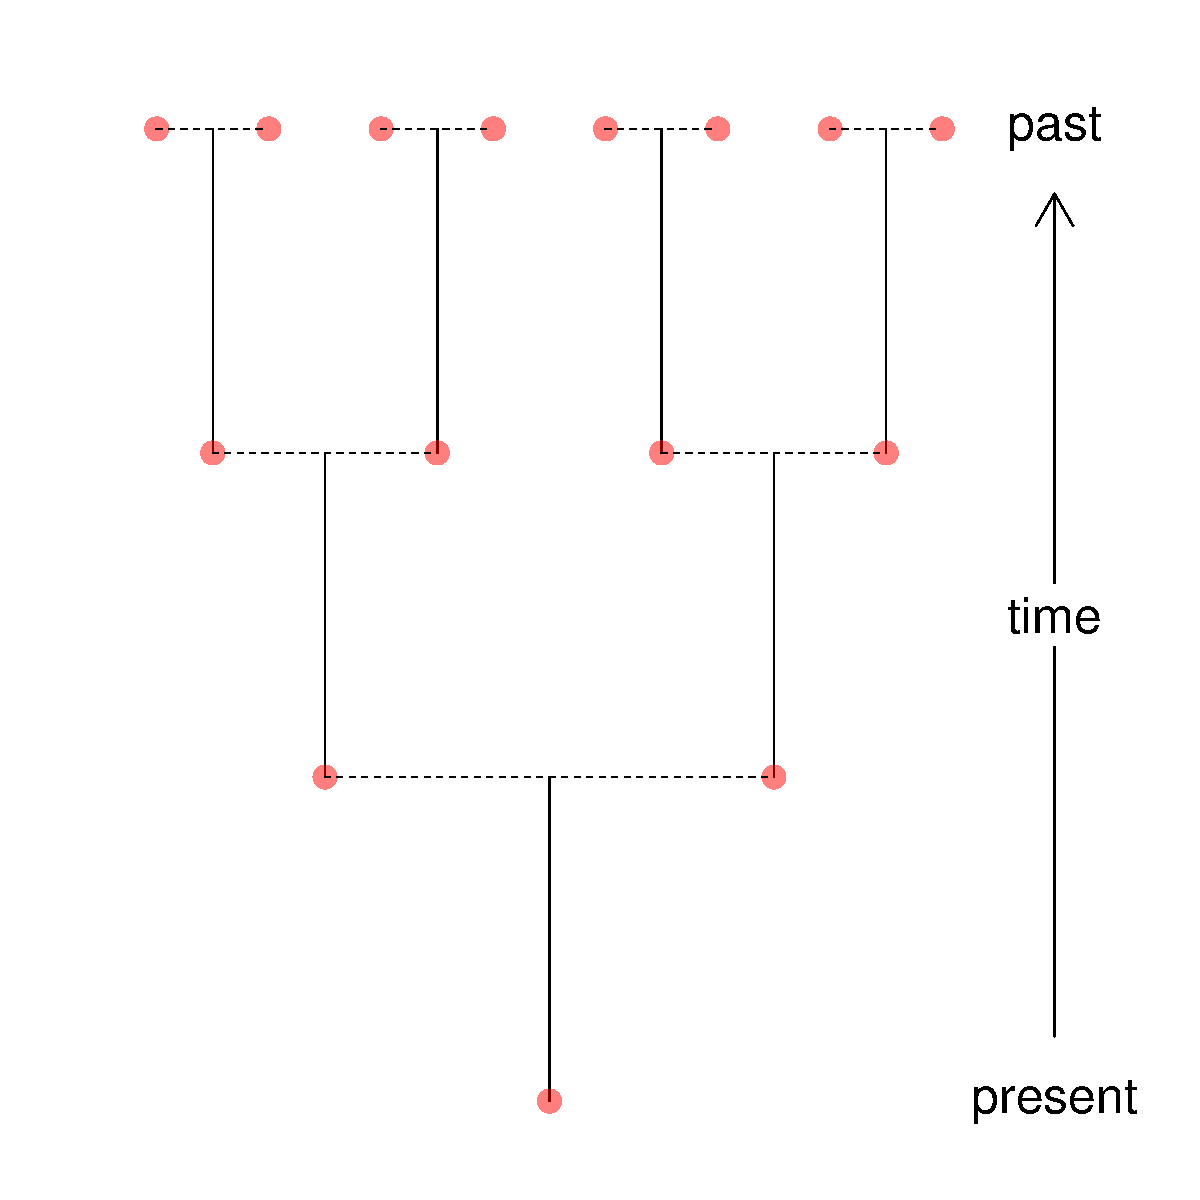
\includegraphics[width=\linewidth]{figs/pedigree.pdf}
        \caption{the pedigree}
        \label{pedigree}
    \end{subfigure}
    \begin{subfigure}{0.55\textwidth}
        \centering 
        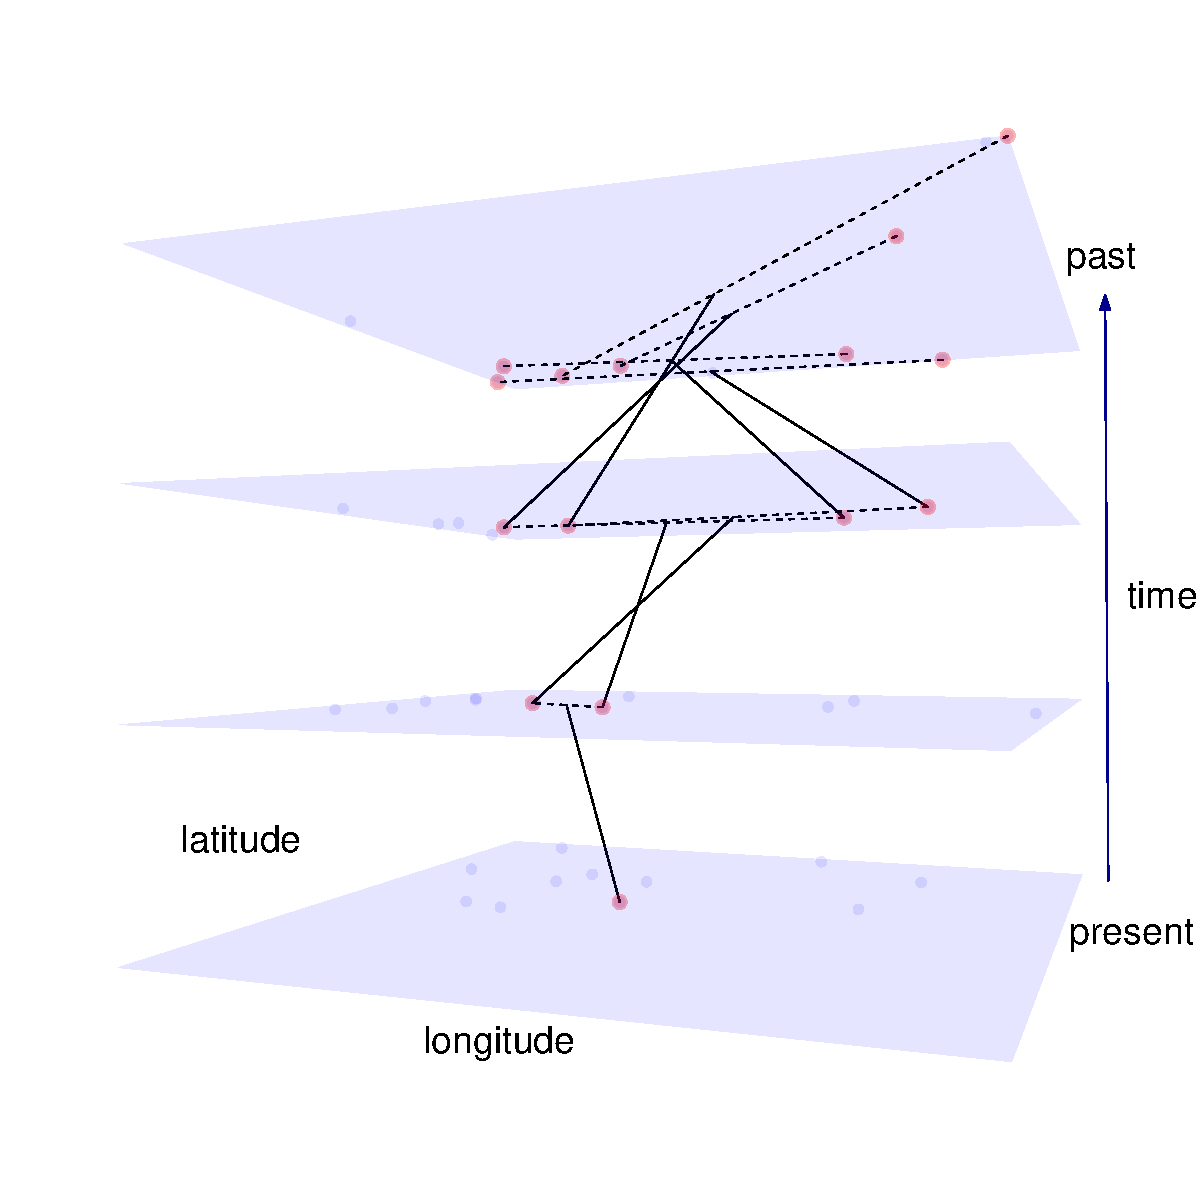
\includegraphics[width=\linewidth]{figs/spatial_pedigree.pdf}
        \caption{the spatial pedigree}
        \label{sp_pedigree}
    \end{subfigure}
        \caption{
            Example spatial pedigree.
                    Each plane represents a a sampled region in a discrete (non-overlapping generation),
                    and each dot represents an individual.
                    The present is at the bottom of the plot, and the past at the top.
                    The spatial pedigree of the ancestors of a focal individual is highlighted in red
                    back through time and across space.
                    Dashed lines denote matings, and solid lines denote parentage.
        }
        \label{spatial_pedigree}
\end{figure}


\section{Things we want to know}
\subsection{Where are they?}

Perhaps the first thing we want to know
when considering a species as a research system
is where they are:
where they can be found, and how many of them there are there.
At finer resolution,
we may also be interested in variation in these counts --
e.g., 
variation in individuals (e.g., how many are reproductive vs. non-reproductive),
or variation in space (more here than there).
%or variation in time (fewer here than there used to be).
Understanding this variation can be crucial for understanding
ecologically important details of a species' natural history,
like whether a particular habitat is a demographic source or sink (Pulliam 1988, Schreiber 2010).
%or how species are responding to anthropogenic climate change (Bi 2013).
The history of abundance and fecundity is recorded in the spatial pedigree,
and we can use data that were generated under this spatial pedigree
to get a peek at the process.

\subsubsection{Population density}

What exactly do we mean by population density?
One definition is simply the number of individuals in a given area,
which is comprehensive,
but may not capture the nuances of natural history we care about.
Ecological modelers interested in population dynamics
may only want to count reproductive adults,
as the average juvenile may not survive to reproduce (e.g. TED paper),
and a non-reproductive adult may not contribute to population growth
(although see helpers at the nest: bee-eaters? acorn woodpeckers?).

An on-the-ground census or a mark-recapture study (ref)
can provide an estimate of the number of individuals in a given region.
This census estimate has the advantage of offering a fairly complete
snapshot of numbers in the modern day,
which may be important for, e.g.,
parameterizing ecological models
or performing environmental impact surveys.
However, these direct census methods have a number of disadvantages as well.
They can be both time- and labor-intensive,
often requiring repeat trips to an area.
In addition, they might not provide information
about the number of reproductive individuals,
and they yield few insights into the numbers of individuals
in an area in the past.

The alternative --
using genetic data to get an estimate of the number of individuals in an area --
can be done using a much smaller number of sampled individuals,
and can offer insights into number of reproductive individuals and historical densities as well.
We can build an intuition for how it is possible to estimate
abundances from genetic data collected from a sample of individuals
using the spatial pedigree generated in scenarios of different abundance.

In an area with a small number of individuals in the each generation
and in a species with short dispersal
(so that there is little influx of migrants from other areas),
the average time to coalescence for a pair of alleles sampled
at random in a generation will be very short.
To see why, consider the relationship between density
and the pool of possible parents.
Each individual in the current generation has two parents that came from nearby,
so in a sparsely populated area,
the pool of individuals who \emph{could} be parents gets exhausted quickly,
and some individuals in the current generation
likely share at least one parent in the previous generation.
If those individuals are not siblings or half-siblings,
they are likely to be recent cousins,
their pedigrees overlapping in this sparsely populated area
in the recent past.

In principle, this is a very simple estimation question:
how many ancestors were there in a given region at a certain time in the past?
However, in addressing this question we quickly run into the familiar
issue of ``effective'' population size.
Information about population sizes in patterns of relatedness
comes from numbers of shared ancestors, i.e., \emph{coalescences}.
The reason for this is simple:
with fewer possible ancestors, the ancestors of two individuals
must be shared more often.
How likely a given individual who lived at some time in the past
is to be a genetic ancestor to a modern-day individual
is just their genetic contribution to the present population.
If we are looking one generation back, this is proportional to their
number of offspring, i.e., their fitness.
If we are looking a long time in the past
(in practice, more than 10 or 20 generations \cite{bartonfitness}),
this is their \emph{long-term fitness}.
The effective population sizes we estimate using coalescence rates
are ``effective'' because of this difference;
to estimate \emph{absolute} population sizes we must take this into account.

        - How many individuals live in a given area? in total?
what exactly do we mean - reproductive adults, or just anyone
If we're trying to infer from the pedigree, we have to be careful bc not everyone leaves genetic descendants
difference between census size and Ne
deeper coalescences in denser areas, more diversity and lower p(IBD)

    -nonreproductive individuals
        -reproductive individuals farther back in the past
    -need to translate between census and effective size


        - How has that number of individuals fluctuated over time? (fast changes as opposed to slow changes)

\plr{figure idea:}
  time slices with circle sizes proportional to eventual genetic contribution, showing increasing imbalance as density of lineages goes from census size to Ne?

\plr{figure idea:} map of heterozygosity across space in a habitat with one big valley surrounded by some small valleys


    -contrast heterogeneity in pedigree relatedness with that of genetic contributions (more in the latter than the former)
   
\subsubsection{Fecundity and reproduction}

How many new offspring are produced per year in a given area? in total?

How do areas contribute in the *long term*?

\plr{figure idea:}
            in an example with higher fecundity in some areas
            (gradient of mean fecundity superimposed on a bumpy landscape?)
            and small bias in dispersal towards lower fecundity area

            * map of population density juxtaposed with
            * a map of per capita number of offspring produced
            * and a map of long-term fitness
         

%%%%%%%%%%%%%%
\subsubsection{Related statistics}

This can be contrasted with a densely populated area,
in which the pool of possible parents in each previous generation is quite large,
so that a random subsample of individuals in the region
will only rarely contain cousins,




There are several ways to look for this signature
of consistently low local abundance
in patterns of population genetic variation.
Diversity statistics, such as Watterson's $\theta$,
will be low



there is a very small pool of local individuals who could
have been the parents of the current generation.
As a result, alleles sampled from individuals in this sparsely populated area
will have short average coalescence times.


It is plausible, and perhaps likely,
that even in a small sample of individuals in the current generation,
a researcher may find siblings or cousins.

If we were only interested in
the modern distribution of all individuals in a species,
we could answer this question by going outside and counting them.
However, we are often also interested in other things as well,
such as just the number of reproductive individuals,
the average fecundity in a particular region,
or in variation in these quantities.
Variation may exist across space,
like when habitats vary in quality
leading to high fecundity in ``good" habitat,
but low fecundity in poor habitat.

     

        - $N_e$
            -Ne now (drift)
    -Ne avg
    -Ne through time
        - census size isn't realized in the genetics, but is relatively
 
    -diversity - chance of nabbing siblings (tract length distns)

%%%%%%%%%%%%%%%%%%%%%%%%%%%%%%
\subsection{How do they move?}

Dispersal is a fundamental process in ecology and evolution,
and is central to many research questions,
including predicting responses to climate change,
evaluating epidemiological networks,
and understanding population demography and dynamics.
Motile organisms move in many ways:
possibly through a day or seasonally through a year,
but quantities we could hope to estimate using population genetic data
have to do with the between-generation \emph{dispersal distance}.
As described above, 
we define the dispersal distance to be the displacement
between parent and offspring birth locations.
The observed distance between parent and offspring
depends on the movement of the parent through its life,
the possible movement of the gamete before fertilization,
the movement of the zygote between formation and maturation,
and daily or seasonal movement of the mature individual,
all of which may depend on the sex of the parent and the offspring.

For some species,
it may be feasible to directly measure many of these components
using, e.g., telemetry or banding \cite{dispersal_estimation}.
However, for most species this will be impractical,
and, as with variation in population density,
measured dispersal of modern individuals in a handful of years
may not be informative short or long-term historical averages
\cite{WhitlockMcCauley1999}.
These processes,
both today and historically,
can be read in the pedigree,
which in turn leaves an imprint on patterns of genetic variation.
If we knew the spatial locations of ancestors in the pedigree,
then realized dispersal would be recorded directly;
we usually do not, but spatial locations of modern individuals
can give strong clues about this \cite{Cayuela2018}.

%%%%%%%%%%%%%%
\subsubsection{Dispersal (individual, diffusive movement; $\sigma$)}

Consider a population living across some geographic area.
One concrete quantity we might be interested in is
the distance between the parent and offspring locations.
To be more careful,
while still trying to stay out of the weeds,
we can define this as the mean distance between the
birth (aka germination/hatching/zygote formation)
location of a randomly chosen parent
and that of one of its randomly chosen offspring.
This notion is actually a cluster of closely related quantities:
for instance, if survival strongly depends on where the offspring disperses to,
then the ``dispersal distance'' estimated by picking an adult from the population
and measuring distance to their offspring (regardless of survival)
could differ from that estimated by measuring the distance between that same adult
and \emph{her} parents.
Suppose the population has been stable forever.
\g{note in Intro about how the field has struggled w/ nonequilibrium dynamics;
we present everything as static first, then revisit these questions in light
of the \emph{very real} possibility that things change through time.}

%Genetic data that come only from adults,
%can never shed light on dispersal distances of offspring that do not survive.

This could be trivially estimated by taking
the average of these displacements across history
if we knew the spatial pedigree through time without error.
In practice, we often are only able to directly observe
the location of individuals in the present day.
However, we can still leverage this information to learn about dispersal distance,
despite not knowing parental locations by
comparing spatial distances between individuals of different levels of relatedness.
For example, if we sample two individuals that are siblings,
then the distance between them is the result of two dispersals,
so an average of this distance over many pairs of siblings gives an estimate of twice the dispersal distance.
First cousins would give four times the dispersal distance, and so forth.
This can be abstracted to any level of relatedness,
however, estimates derived from comparisons of more distantly related individuals
are noisier and more prone to bias.
This is a sort of \emph{sampling bias} --
individuals that live far back in time that do not have descendents today
will not be included in this estimate.
This was nicely summarized by Randall Munroe: ``On the one hand, all my ancestors successfully reproduced; on the other hand, that's the mother of all sampling biases.''

To generalize this type of estimate,
we can correlate the mean time to coalescence between any pair of individuals
with their geographic displacement
to get an estimate of dispersal distance.
In practice,
this is relatively straightforward between close relatives:
long, shared tracts of genome can be used to identify recent cousins,
while identification of more distant relatives is more uncertain.
Nonetheless, how genetic relatedness decays with distance
clearly contains information about dispersal distance.
The mean squared displacement between two individuals
related by a path of total length $n$ through the pedigree
is $\sigma^2 n$,
assuming that $n$ is short enough that boundary effects can be ignored.
If, for $K$ pairs of individuals sampled in the modern day,
we had both known geographic separation $x_1$ through $x_K$
and corresponding degrees of relatedness (i.e., lengths of paths through the pedigree \plr{fixme})
$t_1$ through $t_k$,
then an estimate of squared dispersal distance $\sigma^2$ would be
$\frac{1}{K}\sum_{i=1}^K \|x_i\|^2 / t_i$.
In practice... \cite{Malecot, Barton, Harald}.
\plr{should we talk about collecting/scattering here?}


It may be helpful to think of the dispersal distance
as determining how quickly the population mixes through diffusive movement:
local differentiation between individuals in different parts of the species range
is determined by the balance between drift and gene flow.
If one imagines a spatially restricted allele
as a drop of dye in some water,
the dispersal distance determines how quickly the
color spreads through the water. \plr{move above?}

\plr{figure idea:} ancestry spreading over space

\plr{figure idea:} IBD plot, with points colored/sized according to closest degree of relatedness
(e.g., cousins, second cousins, etc).

\g{figure idea:} two maps, one for a close pair and one for a distant pair, with circles on their MRCAs
with size proportional to amount of genome inherited (and colored according to time?);
this would show the asymptote/collecting phase.

\plr{figure idea:} effective $\sigma$ versus strength of Allee effect

Is there a mean bias (net directionality) in parent-child displacement? Anisotropy?

Male/female differences in dispersal distance?

%%%%%%%%%%%%%%
\subsubsection{Population flux}

The most common summary statistic of dispersal in population genetics
is the average migration rate between a pair of isolated demes.
In continuous space, the analogue of this quantity
is the number of dispersal events that cross
a given boundary each year;
i.e., how many individuals are born each year whose parents
were born on the other side of a given boundary?
\plr{what do we call this? population flux?}
We call this quantity the \emph{population flux} across the boundary,
and it is a useful concept for investigating connectivity between different areas
and the role of the landscape in shaping patterns of dispersal.
For instance,
we might be interested in the flux across a ridgeline between two valleys
relative to that across a similar boundary down the middle of one of the valleys,
which can tell us whether that ridgeline is a substantial barrier to population movement or not.
Note that population flux is not constrained to be equal in both directions across a boundary;
e.g., it may be easier to disperse downhill than uphill,
downwind than upwind,
down-current than up-current, etc..

As before, if we had complete knowledge of the spatial pedigree,
we could calculate the flux across any line simply by counting the number of
parent-offspring pairs that span it.
In practice, we must rely on observations from genetic data,
which introduces two complications.
First, in a given dataset, it is rare to find in one individual
that is a direct ancestor of another in the dataset
(apart from perhaps some parent-child relationships).
Even with historical data (e.g., ancient DNA),
ancient individuals are unlikely to be direct genetic ancestors of modern samples,
and instead are likely to share common genetic ancestors with modern samples.
As a result, we almost never infer dispersal events,
only coalescences between pairs of individuals.
Therefore, the problem of inferring population flux from genetic or genealogical data
cannot be completely disentangled from inferring population density (discussed above).

The second complication is analogous to the problem of effective population size:
the lineages along which genetic material is passed are not an unbiased sample of all dispersal events;
they are weighted by their contribution to the population.
For instance, if there is strong local intra-specific competition,
individuals that dispersed farther from their parents (and their siblings)
may be more likely to reproduce and therefore be represented in the pedigree.
On the other hand, if there is substantial local adaptation,
then many individuals may be dispersing to habitats dissimilar to that of their parents
and are unlikely to transmit genetic material to the next generation
because they are maladapted to the local environment.
(for a review, see \cite{bradburdwang}.)
With sufficient sampling,
it may be possible to get an estimate of flux in the modern sample
that is only minimally affected by these biases.
For example, it may be possible to sample maladapted individuals
before they are picked off,
or to sample individuals in a generation before reproduction.
However, in general, the difference between effective flux and actual flux
will be accentuated the farther back in time one looks.

Effects of sampling design: suppose a big pop is next to a small pop,
since lineages go to the big pop quickly, might need a lot of samples in the small pop
to infer flux well.
Also, if samples are clustered about two points,
we won't really be able to tell if there's a barrier or not,
since all lines we draw between the two are equivalent
from the point of view of our samples.


\plr{figure idea:} adjacent valleys with lower pop density along the intervening ridge,
with arrows denoting all parent-child relationships that cross the ridge
\plr{figure idea:} added to the above, a line drawn down the middle of a valley, with arrows crossing as before (OR, OUT OF A CIRCLE?)

We can use these observations of coalescences to learn about the flux across a given line:
across a barrier to dispersal,
the average time to coalescence for pairs of individuals on opposite sides of the line
is longer than that between individuals on the same side.
Lower population flux means that individuals on opposite sides of a line share ancestors
less frequently.
Also, a barrier means longer across but shorter within coal times \cite{ringbauer2018estimating}.

relationship to dispersal: birth rate times population density times length of boundary times $\sigma/\sqrt{2\pi}$ in each direction
if dispersal is Gaussian and boundary is straight
If the probability of dispersing distance at least $x$ transverse to the boundary is $F(x)$,
in a homogeneous environment with symmetric dispersal,
and population density $\rho$,
the number of individuals crossing the boundary
in a particular direction
per unit of boundary length
is $\int_0^\infty F(x) dx$, where in the integral, $x$ denotes the distance from the boundary.
The mean absolute distance dispersed in a particular direction
(e.g., mean E-W displacement if barrier runs N-S)
is $\mu = \int_0^\infty x F'(x) dx = \int_0^\infty F(x) dx$.
If dispersal is equally likely in any direction,
then $\mu = \E{|X|}$ where $X$ is the dispersal displacement,
since $\sigma^2 = \E{X^2}$, if $X$ is Gaussian then...
\plr{to fix this; this is Buffon's needle}


%%%%%%%%%%%%%%
\subsubsection{Not-resistance surfaces}

Fluxes across lines through the landscape
describe something about population movement,
but are not nearly as satisfying or relevant to researchers
as a map that depicts regions with greater or lesser degrees of population movement.
In heterogeneous environments,
it is clearly desirable to be able to depict local population movement across geography on some kind of a map.
The general description of this kind would be to specify for each location on the map
the probability distribution of where the children of a parent living at that location would end up.
To build an intuition for this,
suppose that in each small section of the map,
we recorded all the dispersals,
how would we describe this collection of dispersal events:
how far they go,
what direction they go,
covariance in noise about that mean.

A way to summarize this by one or a few maps of scalar quantities would be to estimate, at each location, the mean and the covariance of the parent-offspring displacement.
The mean displacement would form a vector field over the map,
where presence of a small arrow would denote some amount of mean bias in offspring dispersal.
The covariance could be summarized by an overall mean distance and a degree of anisotropy.

infinitesimal picture: local mean drift (vector field) and diffusion ellipse leads to amoeboids


%%%%%%%%%%%%%%
\subsubsection{Related statistics}

        - $m$ between "discrete pops"
        - resistance distance


%%%%%%%%%%%%%%
\subsection{Where were their ancestors?}

Above, we have discussed how the dynamics of populations affect
patterns of relatedness,
i.e., how individuals reproduce and move across space.
A complementary view is to
start with individuals sampled in the present day,
then, looking backwards in time,
to ask where their ancestors lived,
and where in space they have inherited their genomes from.
This shifts perspective from moving forwards in the spatial pedigree
(past to present),
to moving backwards in time through it.
As discussed above,
because the signal in genetic data come from shared ancestry and coalescence in the pedigree,
thinking about this perspective is essential to interpreting genetic data.
However, summaries of how ancestry spreads across space through the pedigree can be important in their own right.
For example, humans often have a substantial interest in estimating the locations of their own ancestors
back in time.
More generally,
we are often also interested in the partitioning of genetic diversity across space,
e.g.,
quantifying the strength of inbreeding locally,
or assessing the capacity of a population to become locally adapted.
Spatial locations of ancestry compared across sections of the genome
could also be informative about the origins and mechanisms of selective sweeps.

%%%%%%%%%%
\subsubsection{Geographic distribution of ancestry}

Consider an individual living in a population in a geographic region.
The density of the population back through time and dispersal distance of the ancestors in that individual's pedigree together
determine the rate of spread of that individual's ancestry across space back through time.

Consider a single individual today:
at any point in the past,
each portion of their genome can be associated with the ancestor from whom they inherited that bit of genome.
Their genetic ancestry can therefore be apportioned across space according
to the locations of the ancestors from whom they inherited their genome.
There are a number of natural questions that arise from a description of this process.

For example, we can ask how much of an average individual's ancestry is still within a given region, at some point in the past?
How long in the past was it since a typical individual in one location had an ancestor
in another geographic region (say, the next valley over).
How far back in time do you have to go before the average proportion of ancestry that an individual inherits
from the local region they live in drops below (say) 90\%?

\plr{figure idea:} individuals shaded according to the proportion of ancestry of a given small cluster of samples
they contribute, at several points back in time

%%%%%%%%%%%%
\subsubsection{Geographic distribution of common ancestors}

Take a lineage, follow it back through time
the chance that lineage is in somebody historical is proportional to their long-term fitness
suppose you do that for 2 individuals,
what are the chances that those two coalesce in a particular individual
that's complicated,
but an approximation:
consider a pair of siblings - the chance that those 2 lineages coalesce in a parent of those 2 siblings could be approximated by the product of the long-term fitnesses of those siblings
and a function of the number of offspring of the parent.


This is neat but unclear what it means outside of human-centric whatnot.
White/dark sands lizard example:
if two dunes are separately colonized from dark area but little coalescence happens there
then distribution of MRCAS could be everywhere.

\plr{figure idea:} plot of geographic distribution of mrcas

%%%%%%%%%%%%%%
\subsubsection{(Relative) genetic differentiation}

The question of how genetic variation is partitioned across
geography is a common and intuitively appealing one,
albeit somewhat slippery in practice.
The most common measure of this quantity is $F_{ST}$ \cite{wright},
which measures how much more likely nearby individuals are to share genetic variation than individuals in the population as a whole.
Concretely,
the ratio of mean coalescence time within subpopulations
to that within the entire population measures how closely related
nearby individuals are relative to those in the entire population.
Slatkin (ref) showed that 1 minus this ratio is one way to interpret $F_{ST}$.
This relative genetic differentiation is determined by differing local population densities
and migration fluxes as discussed above:
relative differentiation is determined by the tension between global mixing (due to dispersal)
and local coalescence (due to small population size).
Looking at how ancestry spreads across time and space,
we can see this by looking at how quick it spreads versus coalesces.





        - How much is genetic diversity partitioned across geography?
            How does the expected genetic divergence (or, TMRCA) for nearby individuals compared to distant ones?
         
            * $F_{ST}(x,y) = 1 - (\pi(x,x) + \pi(y,y))/(2 (\pi(x,x) + 2 \pi(x,y) + \pi(y,y)))$,
                i.e., defining mean $F_{ST}$ at distance $x$ to be one minus ratio of mean TMRCA at each location
                to mean TMRCA between individuals from the pops pooled

            * relate to the classic IBD curve

        - How much local inbreeding is there?

            * $\pi(x,x)$? is not heterozygosity, $\pi(x,x)$ should be $\lim_{y \to x} \pi(x,y)$,
                so we can measure this as heterozygosity minus $\pi(x,x)$

refer to figure above of map of heterozygosity



%%%%%%%%%%
\subsubsection{Related statistics}

        - $F_{ST}$, but already covered this

        - relative positions on a PC plot?

%%%%%%%%%%
\subsection{How have things changed over time?}

Each of the questions discussed above -- 
where organisms are; 
how they move;
and where their ancestors were
-- has been introduced under the assumption of a static world 
where species' distributions,
the density of individuals within those species, 
the dispersal patterns of those individuals, 
and the landscape itself all remain constant.
In empirical systems, 
these assumptions are all likely to be broken, 
often drastically so.
Species are expanding into previously unoccupied territory 
all the time;
for example, 
high-latitude tree populations may only have been established 
following the retreat of the glaciers, 
a few tens of generations ago \cite{WhitlockMcCauley1999}, 
and invasive species may have entered their current 
environment even more recently than that (e.g. ref?).
In addition to organisms moving themselves across landscapes, 
landscapes are often changing out from under organisms' feet.
Anthropogenic land use change 
and global climate change 
are both radically altering both where organisms can live 
and where they choose to 
(or even where they \emph{can}) disperse.
Even within a species, 
populations may show spatial discontinuity, 
where most or all the ancestors of the individuals at one location 
lived in another location (eg human refs, Bi 2013).
The result of these changes is that many empirical systems 
are not in equilibrium, 
so that the dynamics we estimate from 
measurements of extant individuals may 
not be representative of those in the past.
Exacerbating this problem, 
the time to reach equilibrium 
in areas of high population density
or across regions of low flux 
may be quite long 
\cite{WhitlockMcCauley1999, CrowAoki1984, Whitlock1992,Slatkin1993}.
%Theory and methods that 
%reflect the empirical reality that things were not always as they are 
%still are lacking, 
Below we discuss different scenarios of nonequilibrium dynamics 
in the spatial pedigree,
and explore how they complicate \g{inference}. 


%%%%%%%%%%
\subsubsection{Identifiability and ill-posedness}

what's the spatiotemporal resolution that you can actually infer things at?
example: fast pop fluctuations just give you lower Ne

%%%%%%%%%%
\subsubsection{Scenario: constant range but more-or-less gradually changing population density due to changing balance of competition/resource availability}

        - Relate to $N_e$-over-time things.

%%%%%%%%%%
\subsubsection{Scenario: postglacial expansion and secondary contact}

        - How much does each individual inherit from each glacial refugium?

            \plr{figure idea:} pie charts of this quantity.

        - Relate to admixture.

%%%%%%%%%%
\subsubsection{Scenario: orogeny induces phylogeny}

        - What proportion of ancestry of one side of the mountain comes from the other side of the mountain,
            as a function of time ago?

           \plr{figure idea:} across a barrier with gradually increasing strength,
                plot of this quantity, compared to if the mountain had not grown.
            -knowlton 1994 snapping shrimp

%%%%%%%%%%
\subsubsection{Scenario: range expansion and exponential growth}

        - Where did the range expansion originate?

        - How fast did it spread?

        - How much surfing was there on the wave front?
       
        - can you tell the difference between source-sink dynamics and a range expansion?

%%%%%%%%%%
\subsubsection{Now is the winter of our discontinuity}

with large-scale range shifts or population movements,
how do you even deal?

%%%%%%%%%%%
\subsection{Are there groups of them?}
One of the first steps in the analysis pipeline of population genetic data
is to quantify and visualize population structure:
systematic differences in genetic similarity between groups of individuals.
Although this can be helpful for generating hypotheses
and, sometimes, for conservation by, e.g., delineating discrete management units,
the concept of discrete population structure
can be problematic or misleading.


Perched on the shoulder of discrete population structure is the concept of admixture,
the idea that populations can be composed of ancestry from multiple discrete groups.
Like discrete population structure,
admixture can offer a useful approximation of reality in some scenarios,
but its utility comes at the cost of ambiguity about what it actually means.

    - Useful for visualization and sometimes management
    
    - but also a crutch, and at times problematic.
    
    - Reality relates to reduced dispersal either today or in the past.


\section{Exciting directions for the field}



%Disclosure
\section*{DISCLOSURE STATEMENT}
If the authors have nothing to disclose, the following statement will be used: The authors are not aware of any affiliations, memberships, funding, or financial holdings that
might be perceived as affecting the objectivity of this review.

% Acknowledgements
\section*{ACKNOWLEDGMENTS}
Brandvain, Marge, JoNo, Graham, Schemske


friendly reviewers: 
Ben Peter? Barton? JoNo? Andy K? Kelleher? Josh Schraiber? Is Petkova still in the mix? 
Etheridge? M Stephens? Harris?

\end{document}




%%%%%%%%%%%%%%%%%%%
%%%%%%%%%%%%%%%%%%%
%
% TEXT GRAVEYARD
%
%%%%%%%%%%%%%%%%%%%
%%%%%%%%%%%%%%%%%%%

Population genetics stands out as a discipline
in which the development of theory was far ahead of empirical possibilities.
Lewontin (1974) described the early state of the field as
``an immensely rich and powerful theory with virtually no suitable facts on which to operate."
For example, the foundations of modern population genetic theory were laid down in XXX,
some XXX years before the first empirical,
molecular measurements of genetic variation were made.
Since then, advances in genotyping and sequencing
have allowed empirical datasets to begin to catch up to theory,
and increasingly, to spur the development of methods to study those new data.
The study of the spatial partitioning of population genetic variation
is an excellent example of this progression.
A large body of early work,
especially that contributed by Wright and Mal\'ecot,
developed theory for populations in an explicit spatial context.
%MORE DETAIL ON THEORY HERE?
%\begin{itemize}
%    \item early theory (continuous and discrete)
%    \begin{itemize}
%        \item wright, malecot, maruyama, nagylaki, felsenstein, slatkin, barton, etheridge, etc.
%                 \item something about isolation by distances and the First Law of Geography (Tobler 1970):
%                    ``everything is related to everything else, but near things are more related than distant things."
%    \end{itemize}
%    \item early empirical popgen out of spatial context (limited by sampling)
%    \begin{itemize}
%        \item e.g., Lewontin and Hubby (``find em and grind em")
%        \item Maybe some stuff on early phenotypable genotypes (pepper moths? )
%        \item chromosomes types (dobzhansky and others)
%        \item But see also wright's work on Linanthes and maybe early stuff on human blood group (cavalli-sforza and others?)
%        \item disconnect between early theory that anticipated the data we'd have now and data then
%\end{itemize}
However, early genotyping methods were limiting.
The earliest empirical measurements of molecular genetic variation
-- the inaugural ``find 'em and grind 'em" work of Lewontin and Hubby (1966) --
focused on data from 43 fly strains sampled from 5 locations,
which were largely treated as experimental replicates
(rather than studied in their geographic context).
Within a decade, genotyping by electrophoresis was being used to quantify
genetic variation in large geographic samples (summarized in Lewontin 1974).
Each subsequent development of a new technique for measuring genetic variation,
starting with counting visible mutations and ending in whole genome re-sequencing,
has followed a similar trajectory from few populations to many.
The major challenge of method development has been
to build models that can keep pace with these new data
to describe the ever greater biological realism and complexity.
Tracing the trajectory of growing richness of empirical datasets,
early methods focused on results in a single panmictic population (ref method?),
then iteratively relaxed the assumption of panmixia with, e.g.,
implementations of the island model (ref method?)
and the stepping-stone model (ref method?).
In reality, well-delineated demes or clearly defined discrete populations are rare.
Rather, organisms are living, moving, reproducing, and dying somewhere in space,
all connected to each other by a pedigree that spans the history of all species.

The current acceleration of empirical sequence generation
has spurred a revolution in the richness of datasets,
which now requires an accompanying revolution in the development of
methods to analyze this wealth of data.
Large and geographically dense samples are now
in genotype-able range in most non-model systems,
and indeed, there are now a handful of populations in which
\emph{every individual} has been sequenced over the past XX generations.
In addition,
the growing ability to genotype historical or ancient individuals
is transforming the study of population genetics,
much of which is predicated on the idea that we can glimpse processes
acting in the past from genetic data obtained from samples in the present,
and for which these direct observations into the past are therefore particularly powerful.
The focus of these datasets has, in many cases,
shifted from discrete populations to the continuous sampling of individuals,
especially within an explicit spatial context.
Taken together, these advances in genotyping make it
an exciting time for method development in population genetics
and, especially, in spatial population genetics.

The field of spatial population genetics is the study of population genetics, in space.
That is, the principal goals of population genetics --
to study patterns of genetic variation within and between populations and
learn about the processes generating those patterns --
are the same as those of spatial population genetics.
However, spatial population genetics as a field is particularly concerned
with the spatial context of these patterns,
leveraging information in the position of samples
to learn about processes governing the distribution of genetic diversity across landscapes.
Spatial population genetics allows researchers
to unite the quantitative descriptions of population genetics
with fundamental questions about the ecology and evolution of organisms.

This review is organized around a definition of the field of spatial population genetics
and its principal applications.
My goal is to provide an introduction for empirical researchers
to the types of questions that can be answered
with spatial population genetics,
and the signals in data that can be used to answer them.
This is a rapidly changing field,
and to a reader of this review five years from now,
many methods currently in use may no longer be relevant
(although hopefully my own contributions will be immortal).
So, rather than discuss the existing methods for inference in detail,
I have instead organized this review around the principal questions in the field
and will focus on the different types of information in genetic and genomic data
that can be brought to bear on those questions.

\section{THE SPATIAL PEDIGREE}
Before diving in, it is useful to define a helpful concept: the spatial pedigree.
The fundamental quantity in the field of population genetics is the ancestral recombination graph (ARG),
which describes the coalescent history of each locus in the genome (argweaver).
This set of gene genealogies is embedded within the pedigree of a species,
in the sense that a pair of sampled alleles cannot coalesce until
the pedigrees of the individuals they are sampled from overlap in a shared ancestor.
The pedigree of a sample is in turn embedded within some spatial context.
Say we start with a sample of two alleles, one from each of two individuals.
If we trace their ancestors across space and back through time,
starting from that focal pair of individuals in the present,
we find that their pedigrees cannot overlap until their ancestors coexist in space.
(The geographic radius within which ancestors can coexist
and pedigrees can overlap is a function of the biology of the specific organism;
broadcast spawners or highly mobile animals can mate over much larger distances than, say, snails.)
Therefore, a useful quantity to consider in the study of
spatial population genetics is the spatial pedigree:
a graph denoting relatedness between all individuals in a sample,
indexed with the geographic position of each individual.
If we had complete knowledge of the spatial pedigree of a species,
including the parentage and location of individuals
who contribute no ancestry to the present-day population,
we would know everything we wished to know of the history of dispersal and gene flow,
population structure and admixture, and selection and fitness in a system.
For example, if we wanted to know the average natal dispersal distance in the species,
we could simply take the mean of the distribution of distances between parents and offspring,
or if we wanted to know the dispersal rate between a pair of locations,
we could count all the times an individual from one dispersed to the other
over the number of generations sampled.
In practice, we never have such a complete understanding of the spatial pedigree,
but it leaves its imprint on different types of genetic and genomic data,
and, by collecting and analyzing these data,
we can try to catch glimpses of it.
SPATIAL PEDIGREE FIGURE

\section{Population Structure and Admixture}
\subsection{What do researchers want to do?}
One of the first steps in the analysis of population genetic data
is to look for and visualize population structure in the sample ?
systematic differences in genetic similarity between groups of individuals.
The goal
This type of analysis can take many forms, such as
dimensionality reduction plots (e.g., PCA, spacemix)
population assignment methods (structure, admixture, conStruct),
population phylogenies (treemix)
plotting pairwise divergence against pairwise geographic distance,
chromosome painting (globetrotter, fineStructure) or ancestry tract inference (Ralph and Coop, Kelly, palamara),
or modeling the site frequency spectrum (dadi, hickerson).
These methods analyze different types of data and employ different models of population history,
but all seek to summarize patterns of genetic variation produced by the spatial pedigree
connecting the individuals in the sample.
Below, I describe different types of population structure,
explain how they arise on the spatial pedigree,
and classify existing methods based on the data they model.

\subsection{What mechanisms underly these patterns on the spatial pedigree?}
Population structure is often well described by a pattern of isolation by distance (Wright),
which is best summed up by the First Law of Geography (Tobler 1970):
``Everything is related to everything else, but near things are more related than distant things."
this pattern emerges from the spatial pedigree when
there is a geographically limited radius within which individuals mate,
and spatial autocorrelation in the geographic positions of parents and offspring.
The result is that individuals farther away from each other in the present
tend not to overlap in their pedigrees until farther back in the past,
leading to higher relatedness between nearby individuals
(wright, barton-etheridge, felsenstein torus, kelleher).
Individuals distributed across a featureless plain in migration-drift equilibrium (Slatkin review)
are expected to exhibit this continuous pattern of isolation by distance.
How quickly this relatedness decays with distance is determined
by the specifics of the biology of an organism:
organisms that move themselves or their gametes over long distances,
and that have high population densities may
exhibit high average relatedness over long spatial lags (Wright 1946).

Sometimes, features of the landscape,
the specific population history,
or quirks of biology
can generate discrete population genetic structure
above and beyond this continuous spatial process.
For example, patchily distributed demes might experience very limited migration (islands, isolated valleys, etc.),
or range expansions might have recently brought two populations that historically
were isolated into close proximity,
and populations in this scenario of secondary contact may
evince some behavioral or intrinsic reproductive isolation.
Although still governed by the same spatial processes,
these scenarios lead to spatial pedigrees in which
the median parent-offspring distance is small relative to the total range.
Note that the mean parent-offspring distance may be much larger
than the median if migrants rarely disperse a long distance,
e.g. between isolated demes (Endler 1977, Rousset 2004).

Admixture is most commonly considered
within the context of discrete population structure,
and is used to describe populations that are composed of ancestry from
multiple discrete groups.
However, admixture can also occur against a backdrop of
continuous geographic structure,
in which case it can be interpreted as relatedness
between the samples from a set of locations
that is unusually high given the geographic distance that separates them (spacemix).
In both continuous and discrete contexts then,
admixture represents a transgressive force,
breaking across population boundaries between discrete demes
or spatial patterns of divergence between distant locations.

In the spatial pedigree,
we describe an individual as ``admixed" when they have recent ancestors
from either a different discrete population or a distant location,
and a population as admixed when many individuals in it share this property.
As has been noted elsewhere (falush, globetrotter, reich),
the ability to identify a population as admixed
is a function of the recency of admixture and
the inclusion of populations descended from the sources of admixture in the modern day sample.
Indeed, the concept of admixture becomes slipperier when considered over deeper timescales,
as inferred sources of admixture are themselves almost certainly admixed,
and have either been isolated for long enough that the admixture is no longer detectable,
or, more likely, the descendants of those sources of admixture are lost in the modern sample.



%FIGURE 2: multipanel figure like Schraiber and Akey Fig 2:
%a) pedigree w/ 3 individuals highlighted (one distant, two nearby)
%b)

\subsection{How do existing methods get at this mechanism?}



\begin{itemize}
\item Estimate Gene Flow and Dispersal
    \item What do researchers want to do?
    \subsubitem
\item The geography of genetic variation
    \item What do researchers want to do?
\end{itemize}





\section{POPULATION STRUCTURE AND ADMIXTURE}
One of the principal aims of spatial population genetics is to describe
and visualize the distribution of genetic variation in a geographic sample.
Most commonly, this means quantifying \emph{population structure} --
systematic differences in genetic similarity between groups of individuals.
Often, population structure is well described by a pattern of isolation by distance (Wright),
which is perhaps best summed up by the First Law of Geography (Tobler 1970):
``Everything is related to everything else, but near things are more related than distant things."
This pattern can be considered under two paradigms:
continuous and discrete.
In the continuous worldview,
population structure is described continuously on a landscape,
by, e.g., considering the rate at which relatedness between individuals decays
with the geographic distance between them.
In the discrete worldview,
population structure is described by defining discrete populations,
within which all individuals are more or less equally related,
and between which there are varying degrees of divergence.
Defined populations may then be used for
management and conservation (``management units" Moritz),
systematics and taxonomy (e.g., describing species or subspecies, ref?)
or delineating evolutionary units of analysis for further study (e.g., GWAS).
These paradigms are often invoked to explain the same
pattern of isolation by distance (IBD),
and, indeed, are not mutually exclusive.
Under both the continuous and discrete worldviews,
individuals or populations can be \emph{admixed}:
composed of a combination of ancestry
from two or more discrete groups or locations.

\subsection{Approaches}
There are a variety of existing approaches for inferring
and visualizing population structure and admixture,
including model-based clustering approaches
(e.g., STRUCTURE, ADMIXTURE, fineStructure, faststructure, tess, geneland, conStruct),
estimating population phylogenies (e.g, TREEMIX,mixmapper?),
reduced-dimensionality analyses (PCA, novembre and stephens, spacemix, SPAmix),
and several heuristics or statistics that range from the simple (Fst, f-statistics)
to the complex (roloff, globetrotter).

These methods employ different models or inference algorithms
and leverage different types of signal
in genetic and genomic data to learn about
the spatial history of population structure and admixture.
To see where that signal comes from,
it is useful to first consider how these processes manifest in the spatial pedigree.

\subsection{Continuous and Discrete Structure, and Admixture}

\paragraph{Continuous Structure}
Continuous, geographically distributed population structure is the simplest to consider:
this pattern emerges from the spatial pedigree when
there is a geographically limited radius within which individuals mate,
and spatial autocorrelation in the geographic positions of parents and offspring.
The result is that individuals farther away from each other in the present
tend not to overlap in their pedigrees until farther back in the past,
leading to higher relatedness between nearby individuals
(wright, barton-etheridge, felsenstein torus, kelleher).

\paragraph{Discrete Structure}
Discrete structure between populations arises
when the coalescent time of alleles sampled
from individuals within a particular group are, on average, lower than
that of a pair of alleles sampled from individuals in different groups (maruyama, nagylaki?).
Because the coalescent is embedded within the pedigree,
this can arise when individuals within a cluster
have more recent pedigree overlap with each other than
they do with individuals between clusters.
Indeed, clusters are defined by this property,
without which ``clusters'' would only be meaningless labels
 randomly assigned to individuals.
In a geographic context, discrete structure is most frequently (and parsimoniously)
ascribed to a reduction in migration between groups
due to geographic separation between patchily distributed demes.
    -something about how this can be due to modern or historical isolation.
        -Note also that equilibrium vs. nonequlibrium
            -for example, discrete population structure can be generated due to historical \emph{or} modern isolation,

\paragraph{Admixture}
Admixture is most commonly considered
within the context of discrete population structure,
and is used to describe populations that are composed of ancestry from
multiple discrete groups.
However, admixture can also occur against a backdrop of
continuous geographic structure,
in which case it can be interpreted as relatedness
between the samples from a set of locations
that is unusually high given the geographic distance that separates them (spacemix).
In both continuous and discrete contexts then,
admixture represents a transgressive force,
breaking across population boundaries between discrete demes
or spatial patterns of divergence between distant locations.

In the spatial pedigree,
we describe an individual as ``admixed" when they have recent ancestors
from either a different discrete population or a distant location,
and a population as admixed when many individuals in it share this property.
As has been noted elsewhere (falush, globetrotter, reich),
the ability to identify a population as admixed
is a function of the recency of admixture and
the inclusion of populations descended from the sources of admixture in the modern day sample.
Indeed, the concept of admixture becomes slipperier when considered over deeper timescales,
as inferred sources of admixture are themselves almost certainly admixed,
and have either been isolated for long enough that the admixture is no longer detectable,
or, more likely, the descendants of those sources of admixture are lost in the modern sample.

\subsection{The Signals in Data}
The pedigree connecting a set of samples under consideration,
along with the geographic position of each ancestor and descendant,
is almost never known;
to identify the signatures left by continuous and discrete population structure and admixture,
we must rely on inferences from patterns of genetic and genomic variation
shaped by the coalescent history embedded within that spatial history.
Methods for detecting population structure and admixture
generally model patterns in one of two types of data:
single-locus and two-locus.

\subsubsection{Single-locus}
In a single-locus analysis,
each locus is treated as an independent draw from the coalescent,
and the data considered are the frequencies of alleles at one or more loci.
These data are generally considered in one of two ways:
patterns of allele frequency divergence or the site frequency spectrum.

\paragraph{Site frequency spectrum}
The site frequency spectrum (SFS) is a summary of population genomic data
that describes the number of derived alleles at a particular frequency
in a sample of individuals.
Under neutrality, and within a panmictic population of constant size,
the proportion of derived alleles found in $i$ out of $n$ genotyped chromosomes
is proportional to $1/i$ (Wakeley).
This expected distribution is derived by considering a mutational process
that drops mutations at random onto the coalescent history of the samples.
In a population of constant size under no selection,
the majority of the length of the coalescent tree is in terminal branches.
The majority of mutations dropped onto this tree at random will therefore be unshared
(only found on a single chromosome).
Relatively few will fall on deeper branches,
which would make them shared by more individuals in the sample.
To develop an intuition for how deviations from panmixia can leave an imprint on the SFS,
it is useful to return to the spatial pedigree and the coalescent it contains.

As described above, discrete population structure in the spatial pedigree manifests as,
on average, more recent pedigree overlap between individuals in the same group
compared to pairs of individuals from different groups.
This leads to a coalescent tree with short intra-group branch lengths
and long inter-group branch lengths,
as individuals in different groups have to go farther back in time until their
ancestors co-occur in the same group and their pedigrees can overlap (nagylaki, maruyama?).
As more of the total tree branch length is in deep branches between groups,
a greater number of mutations on the tree are found in all members of a group,
but not shared between groups,
leading to an unusual number of intermediate-frequency alleles
in the SFS.

SFS in continuous space?
    -no work that I know of
        -presumably shape of SFS is strongly affected by the sampling configuration relative to relevant biological quantities
        -e.g., clumped spatial sampling might be indistinguishable from discrete pop structure
    -a parameterized spatial model should generate an expected coalescent history,
        so I guess you could calculate the likelihood of some observed SFS under a particular spatial model?

Admixture and the SFS?
    -Admixture describes a transgression in the spatial pedigree:
        an ancestor of provenance that is unusual given time and space separating it from its descendant.

-what type of glimpse does the SFS offer into the spatial pedigree?
-Methods that use the SFS

\paragraph{Allele frequency divergence}

Drift and selection act locally to generate differentiation between
discrete populations or locations in continuous space,
and migration acts to homogenize those differences that arise.
Under drift,
the frequency of a given allele at a particular location
is not expected to change through time,
but the variance around that expectation grows with the amount of time
the individuals at that location are isolated,
and the expected difference in the frequency of that allele between
two samples grows (non-linearly) with the amount of isolation between them.
Within populations or locations that are less isolated from each other,
allele frequencies are less free to corkscrew off on independent evolutionary trajectories,
as any changes that arise locally are quickly equalized by migration between them.

Drift is random,
and may be quite slow to differentiate samples if effective population sizes are large,
so the amount of divergence in frequency at any particular locus
may not be informative about their isolation.
However, measured in aggregate across many independent loci,
divergence in allele frequencies can detect even very subtle population structure (Patterson 2006).
Allele frequency divergence offers a glimpse at gene flow averaged
over the history of the spatial pedigree.


-Methods that use allele frequency divergence
 
\paragraph{Two-locus}

In contrast to a single locus analysis,
a two-locus analysis leverages information contained
in the spatial distribution of loci on the genome.


-two locus Methods


\subsection{Spatial Assignment}
    -SCAT (and others?)
    -identifying origins of expansions/invasions
    -estimating wright's neighborhood size

\section{ESTIMATING DISPERSAL AND GENE FLOW}

    \subsection{Identifying barriers and quantifying resistance}
    present: barriers and dispersal (box: gene flow vs. dispersal)
        -IBD-squared, globetrotter, actual pedigrees, MAPS, harald's stuff
            -field of ``landscape genetics"
            -historical data
            -noneq vs. eq
    past: historical migration (and asymmetries)
    -EEMS, BEDASSLE, MAPS, harald's stuff
    \subsection{Inferring demography}
    -SFS models, PSMC/SMSC (covariance in histories)
        -two pop problems vs. many inds
    -colonization/expansion routes
    -identifying invasion sources
    -abundant center hypothesis
\section{THE GENETIC BASIS OF LOCAL ADAPTATION}
    -could also be ``the geography of genetic variation"
        -focus shifts from patterns of divergence in allele frequencies
         to how the frequency of a particular allele is geographically distributred
         (novembre and dirienzo)
             -e.g., skin color alleles, duffy/malaria
    -BAYenv and similar
    -gene dropping down pedigrees, if known
\section{THE FUTURE}
    past - continuity (maybe in 1st section?)
    attempting to infer pedigree (palamara, rasmus, kelly)
    sims (slim and ABC, slim and machine learning)
    cheaper gps tags
    infinite data
 



%\subsection{Gene flow, dispersal, and migration}
%    inds who leave no ancestry may still matter for epidemiological/ecological/conservation
%    Whitlock and McCauley
%    Sokal and Oden 1978
%\subsection{genealogy and geography}
%    -how does pedigree overlap relate to relatedness?

Brief history of work:
\begin{itemize}
    \item early theory (continuous and discrete)
    \begin{itemize}
        \item wright, malecot, maruyama, nagylaki, felsenstein, barton, etheridge
                 \item something about isolation by distances and the First Law of Geography (Tobler 1970):
                    ``everything is related to everything else, but near things are more related than distant things."
    \end{itemize}
    \item early empirical popgen out of spatial context (limited by sampling)
    \begin{itemize}
        \item e.g., Lewontin and Hubby (``find em and grind em")
        \item Maybe some stuff on early phenotypable genotypes (pepper moths?)
        \item But see also wright's work on Linanthes and maybe early stuff on human blood group (cavalli-sforza and others?)
        \item disconnect between early theory that anticipated the data we'd have now and data then
    \end{itemize}
    \item Now lots of theory and methods and datasets,
    \begin{itemize}
        \item but advent of historical/ancient DNA (gamechanger for popgen generally)
            \item  discovery that lots of populations are not continuous through time
        \item drives home a few points:
        \begin{itemize}
            \item we are probably rarely in a migration-drift equilibrium world
            \item genetic variation may be disassociated with geographic context
            \item important to recognize the possibility of heterogeneity of process associated with location through time
        \end{itemize}
    \end{itemize}
        \item Given the availability of these datasets and these advances, I thought it timely to review the blah blah blah
\end{itemize}

FIGURES:
    spatial pedigree
        space, time, pedigree, coalescence, IBD tract, drift
    modern vs. historical isolation (zipping up/zipping down)
    dispersal surfaces AND continuity changing through time

NOTES FROM GRAHAM:
    theory v inference
    one locus v two locus
    one pop to two pops
    marry msmc to harald's stuff

    look at Novembre and DiRienzo paper (2009)
    cavalli-sforza (expansion stuff from pca, or marriage records in Italy, cited in IBD2, harald, or cavalli-sforza remembrances)
    fisher (blood group variants sign of viking invasion)
    mathieson and mcvean pepper moth through time?

    flow from new tech to a small number of pops to a large number of pops (latter of which requires more theory/inference)
    collecting/scattering
 
    dobzhansky's inversion stuff (interested in variation over time vs. space)

NOTES FROM DOUG:
    theory so far ahead of empirical possibilities
    no genotyping, just mendelian traits
    TRYING TO ESTABLISH A SPATIAL NULL
    linanthes perrii (wright's work derived in response to epling's data)
        -wright was only interested in shifting balance
            -expectation of differentiation in space given effective population sizes
            -maybe patterns in linanthes are just explained by drift and differences in pop sizes
            -electrophoresis lead to a rediscovery of Fst, now that they could calculate it
                -annual review by marilyn loveless and jim hamrick - review data for Fst
                    -what plants have high fst?
    collected paper on ecology and evolutionary biology of invasions (grosberg has a paper on it)
        -no evidence for bottlenecking associated invasion
EXTENT TO WHICH GEOGRAPHIC STRUCTURE IN SELECTION IS STRONG ENOUGH TO OVERCOME DRIFT
continuous vs. discontinuous approach (are organisms every truly continuously distributed?)
speciation: geography of speciation
    -linking spatial distribution of adaptive variation to speciation processes
        -how much of the baggage of history is maintained
    -geographic range and range limits
        -range margins (surfing) swamping (kirkpatrick and barton)? running out of variation?
-on methods: what kinds of markers do we need to answer this question?
-using population structure to identify regions under selection
    -nordborg bergelson
    -using clines in allele frequency abundance to identify mechanism of selection?
    -send doug an outline

NOTES FROM BVAIN:
That body of theory has been remarkably useful;
however nearly all of population genetics theory starts with panmictic populations.
It has been tweaked, to accommodate inbreeding and demic structure
(for example, the island model or the stepping-stone model)
This theory has been close and gotten us far
but a major challenge is alligning theory with reality
no populations
no k
just orgs living and dieing and moving in space
and then you can work through ealy ibd
and discrete dems
up to where we are
- build on history to say why we need this
and its exciting
and is to do w data

NOTES FROM PETER:
where are they (make me a map of popn density and mean fecundity)
    -draw a circle on a map and how many inds are int
        if that just's about today, just go count
    -how many have been there over some time,
        -can't just count, but it's recorded in the pedigree
    -
how do they move
what do they do once they're there
are there groups of them?
    -clustering is a crutch that humans use to think
    -could describe all of these (just historical, just ongoing, actual barriers, gnarly source/sink dynamics)
 
 
how has this changed over time
    Barton and Slatkin (hybrid zones, etc.) - nice theory that we can start to get a look at w/ good data
    few notable exceptions (e.g., dobzhansky 1947)
 
    start w/ a barrier, what's happening on a barrier??
    biases in direction of crossing barrier -> expansion/asymmetrical migration and source/sink dynamics, invasion
 
    don't start w/ pop structure, bc what the hell is pop structure
    start w/ something observable like dispersal/migration
 
    mean time to coalescence between two points in space
 
    no one actually cares about the pedigree
        -people want to know how often individuals from A go to B
            -this is answered by the pedigree, but no one actually starts out by asking about the pedigree
 
    start from biology and nonconfusing biological questions
        migration when it's not confusing (islands)
        if we knew where everyone was and what they did
        in practice we can only
     
    barriers and biases in direction
 
    migration, kid-having, population/density
 
    lots of allele A at location 1, could be bc there were originally, or lots of inds go there and don't die, or have lots of kids there
        fitness genetic/geographic correlation
            -context-dependent kid-having

short thing on selection
BISSE problem: if there's lots of allele A at a location, it could be because:
1) lots of inds w/ A go there
2) inds w/ A have more kiddos or die there     less
     
% BITS OF TEXT
Frequently, admixture is described using an \emph{admixture proportion}:
the proportion of genome in a sample that comes from a discrete group,
which is also the probability that an allele taken at random from a sample
come from that group.

I briefly discuss the methods used for answering these questions,
define them in terms of processes shaping the spatial pedigree,
and describe how different types of genetic and genomic data can offer
(sometimes qualitatively) different insights into those processes.

Two revolutions in genotyping technology are leading to
empirical datasets that are more representative of this reality,
which in turn are driving the development of methods to study them.

The first revolution is one of scale.
Setting aside humans and model systems,
for which the wealth of available data and
the rate of generation are simply staggering,
falling sequencing costs are bringing large and geographically dense sampling
into genotype-able range in most non-model systems.
Indeed, there are now a handful of populations in which
\emph{every individual} has been sequenced over the past XX generations,
and the number of populations or species that can make a similar claim
is sure to rise in the near future.
The second revolution is of scope.
The growing ability to genotype historical or ancient individuals
is transforming the study of population genetics,
much of which is predicated on the idea that we can glimpse processes
acting in the past from genetic data obtained from samples in the present.




